\documentclass{article}
\usepackage{pgfplots}
\usepgfplotslibrary{groupplots,fillbetween}
\usepackage{animate}

\begin{document}

 \def\FZero{0}       %x coordinate on Normal distribution you want to project
    \def\Nmu{0.01}      %mu cannot b <= 0
    \def\Nsig{0.25}     %

\pgfmathdeclarefunction{gauss}{2}{%
  \pgfmathparse{1/(#2*sqrt(2*pi))*exp(-((x-#1)^2)/(2*#2^2))}%
}

\pgfmathdeclarefunction{Npdf}{1}{%
  \pgfmathparse{1/(1*sqrt(2*pi))*exp(-((x)^2)/(2*1^2))}%
}

\pgfmathdeclarefunction{logit}{1}{%
  \pgfmathparse{1/(1+exp(-x))}%
}

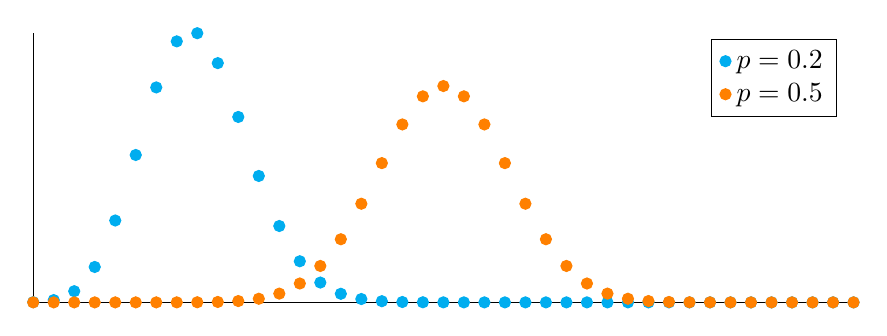
\begin{tikzpicture}[
    declare function={binom(\k,\n,\p)=\n!/(\k!*(\n-\k)!)*\p^\k*(1-\p)^(\n-\k);}
]
\begin{axis}[
    samples at={0,...,40},
  no markers, 
  axis lines*=left,% xlabel=$x$, ylabel=$y$,
  every axis y label/.style={at=(current axis.above origin),anchor=south},
  every axis x label/.style={at=(current axis.right of origin),anchor=west},
  height=5cm, width=12cm,
  xtick=\empty, ytick=\empty, %{4,6.5}
  enlargelimits=false, clip=false, axis on top,
  grid = major 
]
\addplot [only marks, cyan] {binom(x,40,0.2)}; \addlegendentry{$p=0.2$}
\addplot [only marks, orange] {binom(x,40,0.5)}; \addlegendentry{$p=0.5$}
\end{axis}
\end{tikzpicture}

\newpage

 \begin{tikzpicture}
    \begin{groupplot}[
        group style={group size=1 by 3,
                     horizontal sep=0pt,
                     vertical sep=50pt,
                     xticklabels at=edge bottom,
                     yticklabels at=edge left
                     },
                     %customaxis2,
                     height=8cm,
                     width=8cm,
                     legend pos=north east,
    %                grid=both
                     ]
 \nextgroupplot[
  no markers, domain=-3:3, samples=100,
 % axis lines*=left,% xlabel=$x$, ylabel=$y$,
        axis line style={draw=none},
  every axis y label/.style={at=(current axis.above origin),anchor=south},
  every axis x label/.style={at=(current axis.right of origin),anchor=west},
  height=5cm, width=12cm,
  xtick=\empty, ytick=\empty, %{4,6.5}
  enlargelimits=false, clip=false, axis on top,
  grid = major
  ]
  \addplot [very thick,cyan!50!red] {logit({gauss(.25,.65)})};
 \nextgroupplot[
  no markers, domain=-3:3, samples=100,
  %axis lines*=left,% xlabel=$x$, ylabel=$y$,
        axis line style={draw=none},
  every axis y label/.style={at=(current axis.above origin),anchor=south},
  every axis x label/.style={at=(current axis.right of origin),anchor=west},
  height=5cm, width=12cm,
  xtick=\empty, ytick=\empty, %{4,6.5}
  enlargelimits=false, clip=false, axis on top,
  grid = major
  ]
  \addplot [very thick,cyan!50!black] {gauss(.25,.65)};
    \addplot [dashed,cyan!50!black] {gauss(.1,.45)};
    \addplot [dashed,cyan!50!black] {gauss(-1,.4)};
        \addplot [dashed,cyan!50!black] {gauss(1,.75)};
            \addplot [dashed,cyan!50!black] {gauss(-1.5,1)};
                  %    \node[circle,draw] (b1) at (axis cs:{0,0} {};
\nextgroupplot[
  domain=-3:3, samples=100,
 % axis lines*=left,% xlabel=$x$, ylabel=$y$,
       axis line style={draw=none},
  every axis y label/.style={at=(current axis.above origin),anchor=south},
  every axis x label/.style={at=(current axis.right of origin),anchor=west},
  height=5cm, width=12cm,
  xtick=\empty, ytick=\empty, %{4,6.5}
  enlargelimits=false, clip=false, axis on top,
  grid = major
  ]
  \addplot [very thick,cyan!50!black] {gauss(0,1)};
    \end{groupplot}

\end{tikzpicture}



%%%


\end{document}